\section{Expectation-Maximisation (EM) Algorithm}
\label{sec:em}

\paragraph{History}
Although it has been used for parameter estimation of mixture models as early as \citeyear{Newcomb1886} \cite{Newcomb1886}, the \gls{em} algorithm was formally described in a generalised form by \citeauthor{Dempster1977} in \citeyear{Dempster1977}, who also coined the name of the two-step procedure \cite{Dempster1977}. From then on, it has been used in various applications (many of them are described in \cite{McLachlan2008}). In the signal processing community, it has been successfully applied to tasks as diverse as emission tomography image reconstruction \cite{Shepp1982}, active noise cancelling with a single microphone \cite{Feder1989} and parameter estimation of hidden Markov models \cite{Moon1996}. Outside of signal processing, the algorithm is also utilised in many machine learning applications, where it is often introduced as an extended form of the $k$-means algorithm for clustering \cite{Bishop2006}.

% Initialisation
The name \glsentrylong{em} goes back to the algorithm's distinct two steps that both rely on the output of the respective other step. Therefore, prior to the iteration over the E- and M-Step, the estimated parameter set $\bm \theta$ has to be initialised. This initialisation is done randomly in most cases, although one can also include prior knowledge of the estimated parameters by choosing certain initial values for $\theta$ accordingly.

\paragraph{Description} In general, the algorithm allows to determine \gls{ml} estimates or \gls{map} estimates, where only incomplete data is available \cite[p.~1]{Dempster1977}. Incomplete data means that there is a \textit{hidden} or \textit{latent} variable $Z$, that cannot be observed directly but might be inferred by some observable variable $X$. The \textit{complete data} is given by combining the \textit{hidden variable} and the observations.

\paragraph{Derivation}
The cost function of the maximisation problem is the following likelihood function
\begin{equation}
    p(X\given{\theta})=\sum_Z p(X,Z\given{\theta}).
\end{equation}

The assumption is, that maximising $p(X\given{\theta})$ is difficult, but optimisation of the complete data likelihood function $p(X,Z\given{\theta})$ is significantly easier. Next, a distribution $q(Z)$ over the latent variables is defined, which allows, following \cite[p.~450]{Bishop2006}, for the decomposition

\begin{equation}\label{eq:decomposition}
    \ln p(X\given{\theta})=\mathcal{L}(q,\theta)+\text{KL}(q\|p),
\end{equation}

where the summands are defined as
\begin{align}
    \mathcal{L}(q,\theta)&=\sum_Z q(Z)\ln\left\{\frac{p(X,Z\given{\theta})}{q(Z)}\right\}\label{eq:L},\\
    \text{KL}(q\|p)&=-\sum_{Z}q(Z)\ln\left\{\frac{p(Z\given{X,\theta})}{q(Z)} \right\}\label{eq:KL}.
\end{align}

This decomposition can be verified by using the multiplication formula for probabilities, which directly results from the definition of conditional probabilities
\begin{align}
\label{eq:defProbCond}
    p(A\given{B})&=\frac{p(A,B)}{p(B)},\\
\label{eq:defProbProductRule}
    p(A,B)&=p(A\given{B})\cdot p(B).
\end{align}

Applying \eqref{eq:defProbProductRule} to $p(X,Z)$ in \eqref{eq:L} and using the product rule for logarithms $\ln(a\cdot b)=\ln(a)+\ln(b)$ yields

\begin{align}
    \mathcal{L}(q,\theta)&=\sum_{Z}q(Z)\ln\left\{\frac{p(Z\vert X,\theta)\cdot p(X\given{\theta})}{q(Z)}\right\}\\
\label{eq:Lexpanded}
    &=\sum_{Z}q(Z)\ln\left\{\frac{p(Z\given{X,\theta})}{q(Z)} \right\}+\sum_{Z}q(Z)\ln\{p(X\given{\theta})\}.
\end{align}

The first summand is equal to $-\text{KL}(q\|p)$. Therefore it cancels out when inserting \eqref{eq:Lexpanded} back into \eqref{eq:decomposition}. The second summand can be simplified making use of the fact, that $q(Z)$ is a probability distribution and therefore $\sum_{Z}q(Z)=1$ holds true

\begin{align}
    \mathcal{L}(q,\theta)+\text{KL}(q\|p)&=\sum_{Z}q(Z)\ln p(X\given{\theta})-\text{KL}(q\|p)+\text{KL}(q\|p)\\
    &=\ln p(X\given{\theta}).
\end{align}

From \eqref{eq:decomposition} it is apparent, that $\mathcal{L}(q,\theta)$ is a lower bound of $\ln p(X\given{\theta})$, because from $q(Z)>0\ \forall\ Z$ follows KL$(q\|p)\geq0$. In order to maximise the lower bound for a given $\theta^{(l-1)}$, we therefore need to set KL$(q\|p)=0$, so that $\mathcal{L}(q,\theta)=\ln p(X\given{\theta})$. In other words, to compute a lower bound, that is tight with the original likelihood function at $\theta^{(l-1)}$ (i.e. "touches" $\ln p(X\given{\theta})$ in $\theta^{(l-1)}$), we set $\mathcal{L}(q,\theta)=\ln p(X\given{\theta})$, which necessitates
\begin{align}
\label{eq:thatOtherFormulaAbove}
    \text{KL}(q\|p)&=0,\\
    -\sum_{Z}q(Z)\ln\left\{\frac{p(Z\given{X,\theta})}{q(Z)} \right\}&=0.
\label{eq:thatFormulaAbove}
\end{align}

Choosing
\begin{equation}
    q(Z)=p(Z\given{X},\theta)
\label{eq:q}
\end{equation}
satisfies \eqref{eq:thatFormulaAbove}. Inserting \eqref{eq:q} into \eqref{eq:L} and using $\ln(\frac{x}{y})=\ln{x}-\ln{y}$, the lower bound is given by
\begin{align}
    \mathcal{L}(q, \theta)&=\sum_{Z}p(Z\given{X, \theta^{(l-1)}})\ln p(X,Z\given{\theta})-\sum_{Z}p(Z\given{X, \theta^{(l-1)}})\ln p(Z\given{X,\theta^{(l-1)}})\\
    &=\Q+\text{const},
\end{align}

with
\begin{equation}
\label{eq:e-step}
    \Q=\sum_{Z}p(Z\given{X, \theta^{(l-1)}})\ln p(X,Z\given{\theta}).
\end{equation}
    
Computing this lower bound constitutes the E-Step. The M-Step is to find a new value $\theta^{(l)}$, which maximises this lower bound
\begin{equation}
\label{eq:m-step}
    \theta^{(l)} = \argmax_{\theta}\Q.
\end{equation}

\begin{figure}[!hb]
    \centering
    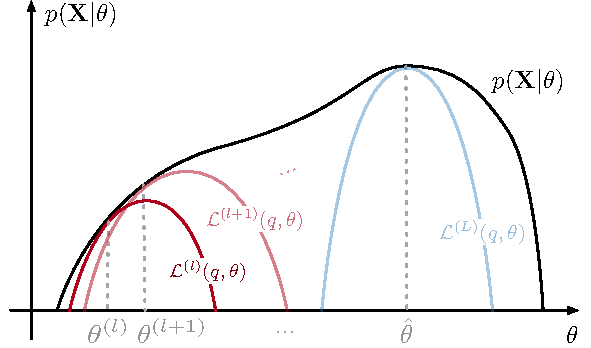
\includegraphics[scale=1]{data/figures/em-Q4}
    \caption[EM-Algorithm as Iterative Lower-bound Optimisation]{EM-Algorithm as Iterative Lower-bound Optimisation.}
    \label{fig:em}
\end{figure}

To summarise, the goal of the E-Step is to find a lower bound for the original, incomplete data likelihood function $p(X\vert\theta)$. This lower bound $\mathcal{L}(q,\bm\theta)$ is chosen to be equal to the original likelihood function in $\theta^{(l-1)}$, which is done by selecting $q(Z)$ to be the posterior probability of the latent variable $Z$ given the observation $X$. This gives rise to the $\mathcal{Q}$-function, which, in the M-Step, is maximised with respects to the estimated parameter set $\bm\theta$. The result is a new value $\bm\theta^{(l)}$, for which a new lower-bound can be found. This procedure is repeated iteratively either until some fixed number of iterations are reached, or some convergence criterion is met. One possible way to determine convergence is to define a lower threshold $\xi$ for the delta of the $\mathcal{Q}$ function. Is the change of $\mathcal{Q}$ from the previous iteration to the current one is lower than or equal to $\xi$, then the algorithm is stopped and $\theta^{(l)}$ is assumed as the solution to the maximum likelihood problem originally stated
\begin{equation}
    \mathcal{Q}(\theta^{(l)}\vert\theta^{(l-1)})-\mathcal{Q}(\theta^{(l-1)}\vert\theta^{(l-2)})\leq\xi.
    \label{eq:convergence-check}
\end{equation}

For a full account of the convergence of \gls{em}, see \cite{Wu1983}. It is interesting to note, that the M-Step only states \textit{that} the result of the E-Step is to be maximised, but not \textit{how} this is to be done. Rather than a specific solution for a certain type of problems, the \gls{em} algorithm is, therefore, more of a template, that can be applied to a variety of different problems, each of them required to individually derive the concrete steps necessary to obtain a lower-bound for the incomplete data log-likelihood function and find it's maximum.

\paragraph{Limitations}
One existing limitation of the \gls{em} algorithm is the possibility of a slow convergence rate, which increases the computational complexity as more iterations have to be carried out before convergence is reached. In this case, the convergence threshold $\xi$ can be increased or replaced by a fixed number of iterations $L$, although this means that the solution is no longer optimal in the \gls{mmse} sense. Another limitation is, that the algorithm is susceptible to local optima for more than one target parameter ($\bm\theta$ is a vector with length $n>1$), meaning that the determined solution is not necessarily the best solution. This can be alleviated by running the algorithm multiple times with a different, random initialisations and choose the best outcome, a procedure known as \textit{random-restart hill climb}. Another method to circumvent getting stuck in local optima is \textit{simulated annealing}, which is incorporated into an \gls{em} template in \cite{Guo2007}. The premise of simulated annealing is to introduce a certain amount of randomness, which allows for the parameter estimate to jump to a neighbouring state (i.e., a different set of parameter estimates) after each iteration. If the neighbouring state is more optimal than the original one, then it is assumed, and estimation is continued with this new state. If the neighbouring state is less optimal in regards to the goal of the optimisation, it is still assumed with a certain probability, which is slowly decreased over time. This allows the algorithm to "escape" local optima at the beginning (when the probability of changing state is high), without losing the ability to converge to an optimum later (when the probability of changing the estimated state is low or even zero).

\begin{figure}[!bh]
    \includegraphics{data/figures/em-flowchart2}
    \caption[Steps of the \glsentryshort{em} algorithm]{Steps of the \glsentryshort{em} algorithm: \itshape The flow-diagram shows the steps of the \gls{em} algorithm and the convergence check after each iteration. Alternatively, a fixed number of iterations $L$ could be set in advance, rendering the check for convergence obsolete.}
\end{figure}

%As KL$(q\|p)$ is the Kullback-Leibler divergence between $q(Z)$ and $p(Z\given{X,\theta})$, it also satisfies KL$(p\|q)\geq 0$ with equality only if $q(Z)=p(Z\given{X,\theta})$. This means, that, using \eqref{eq:decomposition}, we can state, that $\mathcal{L}(q,\theta)$ is a lower bound for the original likelihood function $\ln p(X\given{\theta})$.



%%%%%%%%%%%% OLD STUFF %%%%%%%%%%%%%%%

%\paragraph{Derivation by Andrew Ng, CS229}
%The goal is to maximise the log-likelihood function that is given by
%\begin{equation}\label{eq:likelihood}
%    l(\theta)=\sum_i\log p(x_i;\theta)=\sum_i\log\sum_{z_i} p(x_i,z_i;\theta).
%\end{equation}
%
%Now we assume, that maximising the probability of the observed variable $X$ with respect to the parameter $\theta$ is difficult, but doing this for the probability of the complete data $p(X,Z;theta)$, given by the joint distribution of observed and hidden variables, is easier.
%
%\begin{align}
%    \sum_i \log p(x_i;\theta)&=\sum_i \log \sum_{z_i} p(x_i, z_i;\theta)\\
%          &=\sum_i \log \sum_{z_i} Q_i(z_i)\frac{p(x_i, z_i;\theta)}{Q_i(z_i)}\label{eq:introduce-Q}\\
%          &\geq \sum_i\sum_{z_i}Q_i(z_i)\log\frac{p(x_i,z_i;\theta)}{Q_i(z_i)}\label{eq:lower-bound}
%\end{align}
%
%In \eqref{eq:introduce-Q} we introduced a probability function of the \textit{hidden variable} $Q_i(z_i)$ with the properties $Q_i(z_i)\geq 0\ \forall\ z_i$ and $\sum_{z_i}Q_i(z_i)=1$. This allowed us to use the definition for expectation
%\begin{equation}
%    \sum_{z_i} Q_i(z_i)\frac{p(x_i, z_i;\theta)}{Q_i(z_i)}=E\left\{\frac{p(x_i, z_i;\theta)}{Q_i(z_i)}\right\}
%\end{equation}
%
%and finally use Jensen's inequality
%\begin{align}
%    \text{when\ }f(x) \text{\ is concave:\ }& f(E\{x\}) \geq E\{f(x)\},\label{eq:jensen-concave}\\
%    \text{when\ }f(x) \text{\ is convex:\ }& f(E\{x\}) \leq E\{f(x)\},\label{eq:jensen-convex}
%\end{align}
%
%given that the logarithm is a concave function, which can be shown by
%\begin{equation}
%    \frac{\partial}{\partial x}\log(x)=-\frac{1}{x^2} < 0 \ \forall\ x\in\mathbb{R}^+.
%\end{equation}
%
%Now we have a lower bound \eqref{eq:lower-bound} for the likelihood function \eqref{eq:likelihood}. To define Q we set the constraint, that the lower bound should be as close to the original likelihood function as possible. Therefore, we set the lower bound equal to the original likelihood function for the given parameter $\theta$, which means, that Jensen's inequality needs to be true for the equal case. Combining \eqref{eq:jensen-concave} and \eqref{eq:jensen-convex} shows, that $f(E[x]) = E[f(x)]$ is only true when $f(x)$ is neither concave nor convex, which is only the case for a constant value $f(x) = c\ \forall\ x$. That means
%\begin{equation}
%    \frac{p(x_i,z_i;\theta)}{Q_i(z_i)}=c,
%\end{equation}
%
%which is satisfied, when
%\begin{equation}
%    Q_i(z_i)\propto p(x_i,z_i;\theta).
%\end{equation}
%
%Using the probability distribution property $\sum_{z_i}Q_i(z_i)=1$, we can write
%\begin{align}
%    Q_i(z_i)&=\frac{p(x_i,z_i;\theta)}{\sum_z p(x_i,z;\theta)}\\
%            &=frac{p(x_i,z_i;\theta)}{p(x_i;\theta)}\\
%            &=p(z_i\mid x_i;\theta),
%\end{align}
%
%which is the posterior probability of the hidden variable $z$ given $x$.
%
%In a general form, the two steps of the \gls{em} algorithm are defined as
%
%\subsubsection*{E-Step}
%\begin{equation}\label{eq:e_step_general}
%	Q(\theta,\hat\theta^{(l)})=E_{\hat\theta^{(l)}}\left\{ \log{f_{Y}(y;\theta)\mid z} \right\},
%\end{equation}
%
%\subsubsection*{M-Step}
%\begin{equation}\label{eq:m_step_general}
%	\hat\theta^{(l+1)}=\arg \max_\theta Q\left ( \theta,\hat\theta^{(l)}\right ).
%\end{equation}
%
%%The $Q$-function used in the E-Step can be interpreted as a lower bound of the log-likelihood function to be maximised. To calculate this lower bound, \textit{Jensen's inequality} is used, which states for a concave function $f(x)$ that
%
%The expectation operator is defined as
%\begin{equation}\label{eg:expectation-definition}
%    E\{f(x)\}=\sum_x f(x)P(x),
%\end{equation}
%
%Bringing this all together, we are now able to determine a lower bound for the log likelihood function
%\begin{equation}
%    \log\left(\sum_x f(x)P(x)\right) \leq \sum_x \log f(x)P(x),
%\end{equation}